\documentclass[12pt, oneside]{article}

\usepackage[letterpaper, scale=0.89, centering]{geometry}
\usepackage{fancyhdr}
\setlength{\parindent}{0em}
\setlength{\parskip}{1em}

\usepackage{tikz}
\usetikzlibrary{automata,positioning,arrows}

\pagestyle{fancy}
\fancyhf{}
\renewcommand{\headrulewidth}{0pt}
\rfoot{\href{https://creativecommons.org/licenses/by-nc-sa/2.0/}{CC BY-NC-SA 2.0} Version \today~(\thepage)}

\usepackage{amssymb,amsmath,pifont,amsfonts,comment,enumerate,enumitem}
\usepackage{currfile,xstring,hyperref,tabularx,graphicx,wasysym}
\usepackage[labelformat=empty]{caption}
\usepackage{xcolor}
\usepackage{multicol,multirow,array,listings,tabularx,lastpage,textcomp,booktabs}

% NOTE(joe): This environment is credit @pnpo (https://tex.stackexchange.com/a/218450)
\lstnewenvironment{algorithm}[1][] %defines the algorithm listing environment
{   
    \lstset{ %this is the stype
        mathescape=true,
        frame=tB,
        numbers=left, 
        numberstyle=\tiny,
        basicstyle=\rmfamily\scriptsize, 
        keywordstyle=\color{black}\bfseries,
        keywords={,procedure, div, for, to, input, output, return, datatype, function, in, if, else, foreach, while, begin, end, }
        numbers=left,
        xleftmargin=.04\textwidth,
        #1
    }
}
{}

\newcommand\abs[1]{\lvert~#1~\rvert}
\newcommand{\st}{\mid}

\newcommand{\cmark}{\ding{51}}
\newcommand{\xmark}{\ding{55}}


\begin{document}
\begin{flushright}
    \StrBefore{\currfilename}{.}
\end{flushright}

\section*{Monday: Turing machines}

%! app: Decidable Languages, Undecidable Languages
%! outcome: Formal definition of automata, Informal definition of automata, Classify language, Find example languages

For Turing machine $M= (Q, \Sigma, \Gamma, \delta, q_0, q_{accept}, q_{reject})$ 
where $\delta$ is the {\bf transition function} 
\[
  \delta: Q\times \Gamma \to Q \times \Gamma \times \{L, R\}
\]
the {\bf computation} of $M$ on a string $w$ over $\Sigma$  is:

\begin{itemize}
\setlength{\itemsep}{0pt}
\item Read/write head starts at leftmost position on tape. 
\item Input string is written on $|w|$-many leftmost cells of tape, 
rest of  the tape cells have  the blank symbol. {\bf Tape alphabet} 
is $\Gamma$ with $\textvisiblespace\in \Gamma$ and $\Sigma \subseteq \Gamma$.
The blank symbol $\textvisiblespace \notin \Sigma$.
\item Given current state of machine and current symbol being read at the tape head, 
the machine transitions to next state, writes a symbol to the current position  of the 
tape  head (overwriting existing symbol), and moves the tape head L or R (if possible). 
\item Computation ends {\bf if and when} machine enters either the accept or the reject state.
This is called {\bf halting}.
Note: $q_{accept} \neq q_{reject}$.
\end{itemize}

The {\bf language recognized by the  Turing machine} $M$,  is  $L(M) = \{ w \in \Sigma^* \mid w \textrm{ is accepted by } M\}$,
which is defined as
\[
  \{ w \in \Sigma^* \mid \textrm{computation of $M$ on $w$ halts after entering the accept state}\}
\]
  
\newpage
\begin{multicols}{2}
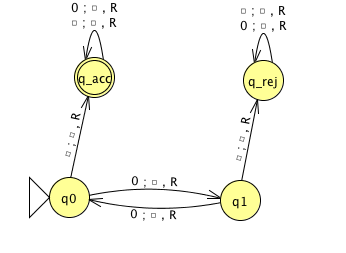
\includegraphics[width=2.5in]{../../resources/machines/Lect13TM1.png}

\columnbreak
Formal definition:

\vspace{10pt}

Sample computation: 

\begin{tabular}{|c|c|c|c|c|c|c|}
\hline
\multicolumn{1}{|c}{$q0\downarrow$} &  \multicolumn{6}{c|}{\phantom{A}}\\
\hline
$0$ & $0$  & $0$ & $\textvisiblespace $& $\textvisiblespace $& $\textvisiblespace $&  $\textvisiblespace $\\
\hline
\multicolumn{7}{|c|}{\phantom{A}}\\
\hline
\phantom{AA} & \phantom{AA}& \phantom{AA}& \phantom{AA}& \phantom{AA}& \phantom{AA}& \phantom{AA} \\
\hline
\multicolumn{7}{|c|}{\phantom{A}}\\
\hline
\phantom{AA} & \phantom{AA}& \phantom{AA}& \phantom{AA}& \phantom{AA}& \phantom{AA}& \phantom{AA} \\
\hline
\multicolumn{7}{|c|}{\phantom{A}}\\
\hline
\phantom{AA} & \phantom{AA}& \phantom{AA}& \phantom{AA}& \phantom{AA}& \phantom{AA}& \phantom{AA} \\
\hline
\multicolumn{7}{|c|}{\phantom{A}}\\
\hline
\phantom{AA} & \phantom{AA}& \phantom{AA}& \phantom{AA}& \phantom{AA}& \phantom{AA}& \phantom{AA} \\
\hline
\end{tabular}
\end{multicols}
\vfill

The language recognized by this machine is \ldots

\vfill


To define a Turing machine, we could give a 
\begin{itemize}
\item {\bf Formal definition}, namely the $7$-tuple of parameters including set of states, 
input alphabet, tape alphabet, transition function, start state, accept state, and reject state; or,
\item {\bf Implementation-level definition}: English prose that describes the Turing machine head 
movements relative to contents of tape, and conditions for accepting / rejecting based on those contents.
\end{itemize}

Conventions for drawing state diagrams of Turing machines: (1) omit the reject state from the diagram (unless 
it's the  start state), (2) any missing transitions in the state diagram have value $(q_{reject}, ~\textvisiblespace~ , R)$.
\newpage

{\it Sipser Figure  3.10}
\begin{multicols}{2}
\vspace{-20pt}
\begin{center}
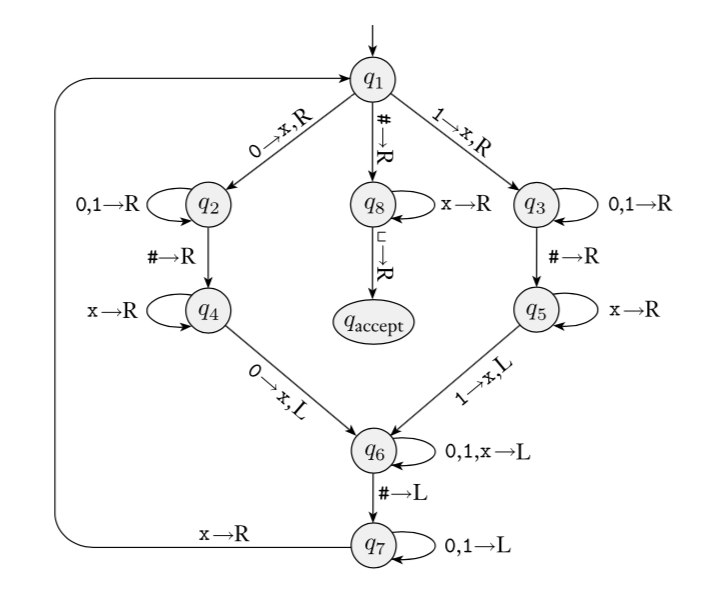
\includegraphics[width=4in]{../../resources/machines/Lect13TM3.png}
\end{center}

Implementation level description of this machine:
\begin{quote}
Zig-zag across tape to corresponding positions on either side of $\#$ to check whether the 
characters in these positions agree. If they do not, or if there is no $\#$, reject. If they 
do, cross them off.

Once all symbols to the left of the $\#$ are crossed off, check for any un-crossed-off symbols 
to the right of $\#$; if there are any, reject; if there aren't, accept.
\end{quote}

\columnbreak

Computation on  input  string  $01\#01$

\begin{tabular}{|c|c|c|c|c|c|c|}
\hline
\multicolumn{1}{|c}{$q_1 \downarrow$} &  \multicolumn{6}{c|}{\phantom{A}}\\
\hline
$0$ & $1$  & $\#$  & $0$ & $1$ & $\textvisiblespace $& $\textvisiblespace $\\
\hline
  \multicolumn{7}{|c|}{\phantom{A}}\\
  \hline
  \phantom{AA} & \phantom{AA}& \phantom{AA}& \phantom{AA}& \phantom{AA}& \phantom{AA}& \phantom{AA} \\
  \hline
  \multicolumn{7}{|c|}{\phantom{A}}\\
  \hline
  \phantom{AA} & \phantom{AA}& \phantom{AA}& \phantom{AA}& \phantom{AA}& \phantom{AA}& \phantom{AA} \\
  \hline
  \multicolumn{7}{|c|}{\phantom{A}}\\
  \hline
  \phantom{AA} & \phantom{AA}& \phantom{AA}& \phantom{AA}& \phantom{AA}& \phantom{AA}& \phantom{AA} \\
  \hline
  \multicolumn{7}{|c|}{\phantom{A}}\\
  \hline
  \phantom{AA} & \phantom{AA}& \phantom{AA}& \phantom{AA}& \phantom{AA}& \phantom{AA}& \phantom{AA} \\
  \hline
  \multicolumn{7}{|c|}{\phantom{A}}\\
  \hline
  \phantom{AA} & \phantom{AA}& \phantom{AA}& \phantom{AA}& \phantom{AA}& \phantom{AA}& \phantom{AA} \\
  \hline
  \multicolumn{7}{|c|}{\phantom{A}}\\
  \hline
  \phantom{AA} & \phantom{AA}& \phantom{AA}& \phantom{AA}& \phantom{AA}& \phantom{AA}& \phantom{AA} \\
  \hline
  \multicolumn{7}{|c|}{\phantom{A}}\\
  \hline
  \phantom{AA} & \phantom{AA}& \phantom{AA}& \phantom{AA}& \phantom{AA}& \phantom{AA}& \phantom{AA} \\
  \hline
  \multicolumn{7}{|c|}{\phantom{A}}\\
  \hline
  \phantom{AA} & \phantom{AA}& \phantom{AA}& \phantom{AA}& \phantom{AA}& \phantom{AA}& \phantom{AA} \\
  \hline
  \multicolumn{7}{|c|}{\phantom{A}}\\
  \hline
  \phantom{AA} & \phantom{AA}& \phantom{AA}& \phantom{AA}& \phantom{AA}& \phantom{AA}& \phantom{AA} \\
  \hline
  \multicolumn{7}{|c|}{\phantom{A}}\\
  \hline
  \phantom{AA} & \phantom{AA}& \phantom{AA}& \phantom{AA}& \phantom{AA}& \phantom{AA}& \phantom{AA} \\
  \hline
  \multicolumn{7}{|c|}{\phantom{A}}\\
  \hline
  \phantom{AA} & \phantom{AA}& \phantom{AA}& \phantom{AA}& \phantom{AA}& \phantom{AA}& \phantom{AA} \\
  \hline
  \multicolumn{7}{|c|}{\phantom{A}}\\
  \hline
  \phantom{AA} & \phantom{AA}& \phantom{AA}& \phantom{AA}& \phantom{AA}& \phantom{AA}& \phantom{AA} \\
  \hline
  \multicolumn{7}{|c|}{\phantom{A}}\\
  \hline
  \phantom{AA} & \phantom{AA}& \phantom{AA}& \phantom{AA}& \phantom{AA}& \phantom{AA}& \phantom{AA} \\
  \hline
  \multicolumn{7}{|c|}{\phantom{A}}\\
  \hline
  \phantom{AA} & \phantom{AA}& \phantom{AA}& \phantom{AA}& \phantom{AA}& \phantom{AA}& \phantom{AA} \\
  \hline
  \multicolumn{7}{|c|}{\phantom{A}}\\
  \hline
  \phantom{AA} & \phantom{AA}& \phantom{AA}& \phantom{AA}& \phantom{AA}& \phantom{AA}& \phantom{AA} \\
  \hline
  \multicolumn{7}{|c|}{\phantom{A}}\\
  \hline
  \phantom{AA} & \phantom{AA}& \phantom{AA}& \phantom{AA}& \phantom{AA}& \phantom{AA}& \phantom{AA} \\
  \hline
  \multicolumn{7}{|c|}{\phantom{A}}\\
  \hline
  \phantom{AA} & \phantom{AA}& \phantom{AA}& \phantom{AA}& \phantom{AA}& \phantom{AA}& \phantom{AA} \\
  \hline
  \multicolumn{7}{|c|}{\phantom{A}}\\
  \hline
  \phantom{AA} & \phantom{AA}& \phantom{AA}& \phantom{AA}& \phantom{AA}& \phantom{AA}& \phantom{AA} \\
  \hline
  \end{tabular}
\end{multicols}


The language recognized by this machine is
\[
  \{ w \# w \mid w \in \{0,1\}^* \}
\]

\newpage
{\it Extra practice}

Computation on  input  string  $01\#1$

\begin{tabular}{|c|c|c|c|c|c|c|}
\hline
\multicolumn{1}{|c}{$q_1\downarrow$} &  \multicolumn{6}{c|}{\phantom{A}}\\
\hline
$0$ & $1$  & $\#$  & $1$ & $\textvisiblespace $& $\textvisiblespace $&  $\textvisiblespace $\\
\hline
\multicolumn{7}{|c|}{\phantom{A}}\\
\hline
\phantom{AA} & \phantom{AA}& \phantom{AA}& \phantom{AA}& \phantom{AA}& \phantom{AA}& \phantom{AA} \\
\hline
\multicolumn{7}{|c|}{\phantom{A}}\\
\hline
\phantom{AA} & \phantom{AA}& \phantom{AA}& \phantom{AA}& \phantom{AA}& \phantom{AA}& \phantom{AA} \\
\hline
\multicolumn{7}{|c|}{\phantom{A}}\\
\hline
\phantom{AA} & \phantom{AA}& \phantom{AA}& \phantom{AA}& \phantom{AA}& \phantom{AA}& \phantom{AA} \\
\hline
\multicolumn{7}{|c|}{\phantom{A}}\\
\hline
\phantom{AA} & \phantom{AA}& \phantom{AA}& \phantom{AA}& \phantom{AA}& \phantom{AA}& \phantom{AA} \\
\hline
\multicolumn{7}{|c|}{\phantom{A}}\\
\hline
\phantom{AA} & \phantom{AA}& \phantom{AA}& \phantom{AA}& \phantom{AA}& \phantom{AA}& \phantom{AA} \\
\hline
\multicolumn{7}{|c|}{\phantom{A}}\\
\hline
\phantom{AA} & \phantom{AA}& \phantom{AA}& \phantom{AA}& \phantom{AA}& \phantom{AA}& \phantom{AA} \\
\hline
\multicolumn{7}{|c|}{\phantom{A}}\\
\hline
\phantom{AA} & \phantom{AA}& \phantom{AA}& \phantom{AA}& \phantom{AA}& \phantom{AA}& \phantom{AA} \\
\hline
\multicolumn{7}{|c|}{\phantom{A}}\\
\hline
\phantom{AA} & \phantom{AA}& \phantom{AA}& \phantom{AA}& \phantom{AA}& \phantom{AA}& \phantom{AA} \\
\hline
\multicolumn{7}{|c|}{\phantom{A}}\\
\hline
\phantom{AA} & \phantom{AA}& \phantom{AA}& \phantom{AA}& \phantom{AA}& \phantom{AA}& \phantom{AA} \\
\hline
\multicolumn{7}{|c|}{\phantom{A}}\\
\hline
\phantom{AA} & \phantom{AA}& \phantom{AA}& \phantom{AA}& \phantom{AA}& \phantom{AA}& \phantom{AA} \\
\hline
\multicolumn{7}{|c|}{\phantom{A}}\\
\hline
\phantom{AA} & \phantom{AA}& \phantom{AA}& \phantom{AA}& \phantom{AA}& \phantom{AA}& \phantom{AA} \\
\hline
\multicolumn{7}{|c|}{\phantom{A}}\\
\hline
\phantom{AA} & \phantom{AA}& \phantom{AA}& \phantom{AA}& \phantom{AA}& \phantom{AA}& \phantom{AA} \\
\hline
\multicolumn{7}{|c|}{\phantom{A}}\\
\hline
\phantom{AA} & \phantom{AA}& \phantom{AA}& \phantom{AA}& \phantom{AA}& \phantom{AA}& \phantom{AA} \\
\hline
\multicolumn{7}{|c|}{\phantom{A}}\\
\hline
\phantom{AA} & \phantom{AA}& \phantom{AA}& \phantom{AA}& \phantom{AA}& \phantom{AA}& \phantom{AA} \\
\hline
\multicolumn{7}{|c|}{\phantom{A}}\\
\hline
\phantom{AA} & \phantom{AA}& \phantom{AA}& \phantom{AA}& \phantom{AA}& \phantom{AA}& \phantom{AA} \\
\hline
\multicolumn{7}{|c|}{\phantom{A}}\\
\hline
\phantom{AA} & \phantom{AA}& \phantom{AA}& \phantom{AA}& \phantom{AA}& \phantom{AA}& \phantom{AA} \\
\hline
\multicolumn{7}{|c|}{\phantom{A}}\\
\hline
\phantom{AA} & \phantom{AA}& \phantom{AA}& \phantom{AA}& \phantom{AA}& \phantom{AA}& \phantom{AA} \\
\hline
\multicolumn{7}{|c|}{\phantom{A}}\\
\hline
\phantom{AA} & \phantom{AA}& \phantom{AA}& \phantom{AA}& \phantom{AA}& \phantom{AA}& \phantom{AA} \\
\hline
\multicolumn{7}{|c|}{\phantom{A}}\\
\hline
\phantom{AA} & \phantom{AA}& \phantom{AA}& \phantom{AA}& \phantom{AA}& \phantom{AA}& \phantom{AA} \\
\hline
\multicolumn{7}{|c|}{\phantom{A}}\\
\hline
\phantom{AA} & \phantom{AA}& \phantom{AA}& \phantom{AA}& \phantom{AA}& \phantom{AA}& \phantom{AA} \\
\hline
\end{tabular}


    
\newpage
\subsection*{Wednesday: Describing Turing machines and algorithms}

%! app: decidable languages, undecidable languages
%! outcome: Formal definition of automata, Informal definition of automata, Classify language, Find example languages
    
Two models of computation are called {\bf equally expressive} when 
every language recognizable with the first model is recognizable with the second, and vice versa.

True / False: NFAs and PDAs are equally expressive.

True / False: Regular expressions and CFGs are equally expressive.


\begin{center}
{\large \it  Some examples of models that are {\bf equally expressive} with deterministic Turing machines: }
\end{center}

\fbox{ {\bf May-stay}  machines }
The May-stay machine model is the same as the usual Turing machine model,  except that
on each transition, the tape head may move L, move R, or Stay. 

Formally: $(Q, \Sigma, \Gamma, \delta, q_0, q_{accept}, q_{reject})$ where 
\[
  \delta: Q \times \Gamma \to Q \times \Gamma \times \{L, R, S\}
\]

{\bf Claim}: Turing machines and May-stay machines are equally expressive. {\it To prove \ldots}

To translate a standard TM to a may-stay machine: 

\vspace{100pt}




To translate one  of the  may-stay machines to standard TM:
any time TM would Stay, move right  then  left.


Formally: suppose $M_S =  (Q, \Sigma, \Gamma, \delta, q_0, q_{acc}, q_{rej})$
has $\delta: Q \times \Gamma \to Q \times \Gamma \times \{L, R, S\}$. Define
the Turing-machine
\[
  M_{new} =  (\phantom{\hspace{2.5in}})
\]

\vfill

\newpage

\phantom{$M_{new}$ construction here \vspace{400pt}}
\vfill


\fbox{ {\bf Multitape Turing machine}} A multitape Turing macihne with $k$ tapes
can be formally representated as 
$(Q, \Sigma,  \Gamma, \delta, q_0, q_{acc}, q_{rej})$ 
where $Q$ is the finite set of  states,
$\Sigma$ is the  input alphabet with  $\textvisiblespace \notin \Sigma$,
$\Gamma$  is the  tape alphabet with $\Sigma \subsetneq \Gamma$ ,
$\delta: Q\times \Gamma^k\to Q \times \Gamma^k \times \{L,R\}^k$ 
(where $k$ is  the number of  states)


If $M$ is a standard  TM, it is a $1$-tape machine.


To translate a $k$-tape machine  to  a standard TM:
Use a  new symbol to separate the contents of each tape
and keep track of location of  head with  special version of each
tape symbol. {\tiny Sipser Theorem 3.13} 

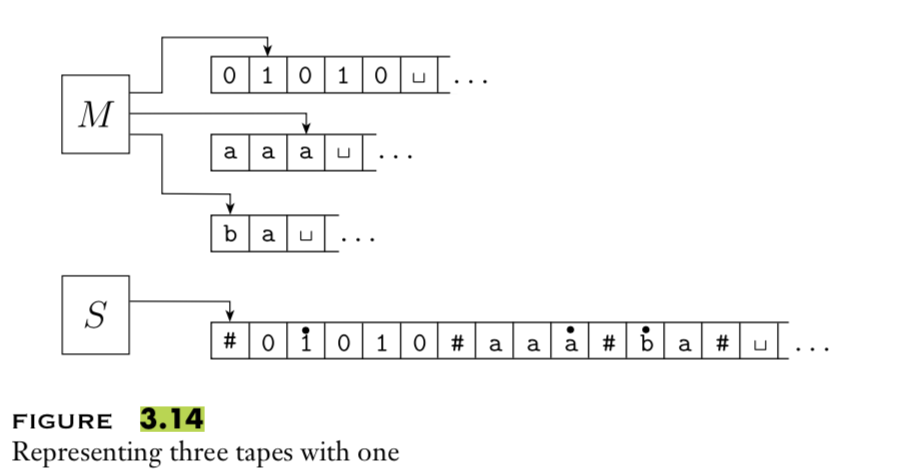
\includegraphics[width=2.5in]{../../resources/images/Figure314.png}


{\it Extra practice:} \fbox{ {\bf  Wikipedia Turing machine} }
Define a machine $(Q, \Gamma, b, \Sigma,  q_0, F, \delta)$
where $Q$ is the finite set  of  states
$\Gamma$  is the tape alphabet,
$b \in \Gamma$ is the blank symbol, 
$\Sigma \subsetneq \Gamma$ is the  input alphabet, 
$q_0 \in  Q$ is the start state, 
$F \subseteq Q$ is the set of accept states, 
$\delta: (Q \setminus F)  \times  \Gamma \not\to Q \times  \Gamma  \times \{L, R\}$
 is a partial transition function
If computation enters a state  in $F$, it  accepts 
If computation enters a configuration where
 $\delta$ is not defined, it  rejects . {\tiny Hopcroft and  Ullman, cited by  Wikipedia} 

\newpage
\fbox{ {\bf Enumerators} } Enumerators give a different
model of computation where a language is {\bf produced, one string at a time},
rather than recognized by accepting (or not) individual strings.

Each enumerator machine has finite state control, unlimited work tape, and a printer. The computation proceeds
according to transition function; at any point machine may ``send'' a string to the printer.
\[
E  = (Q, \Sigma, \Gamma, \delta, q_0, q_{print})  
\]
$Q$ is the finite set of states, $\Sigma$ is  the output alphabet, $\Gamma$ is the 
tape alphabet ($\Sigma  \subsetneq\Gamma, 
\textvisiblespace \in \Gamma \setminus \Sigma$), 
\[
\delta:  Q  \times  \Gamma \times \Gamma \to  Q \times  \Gamma \times  \Gamma \times \{L, R\} \times  \{L, R\}
\]
where in state $q$, when the working tape is scanning character $x$ and the printer tape is scanning character $y$,
$\delta( (q,x,y) ) = (q', x', y', d_w, d_p)$ means transition to control state $q'$, write $x'$ on 
the working tape, write $y'$ on the printer tape, move in direction $d_w$ on the working tape, and move in direction 
$d_p$ on the printer tape. The computation starts in $q_0$ and each time the computation enters $q_{print}$
the string from the leftmost edge of the printer tape to the first blank cell is considered to be printed.

The language  {\bf  enumerated} by  $E$, $L(E)$, is $\{ w \in \Sigma^* \mid \text{$E$ eventually, at finite  time, 
prints $w$} \}$.


\begin{center}
\begin{tabular}{cc}
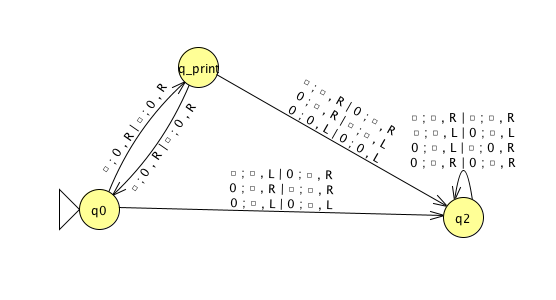
\includegraphics[width=3.5in]{../../resources/machines/Lec15enumerator.png}  & 
\begin{tabular}{|c|c|c|c|c|c|c|}
\hline
\multicolumn{1}{|c}{$q0$} &  \multicolumn{6}{c|}{\phantom{A}}\\
\hline
$\textvisiblespace ~*$& $\textvisiblespace$  & $\textvisiblespace$ & $\textvisiblespace$& $\textvisiblespace$& $\textvisiblespace$&  $\textvisiblespace$\\
\hline
$\textvisiblespace  ~*$& $\textvisiblespace$  & $\textvisiblespace$ & $\textvisiblespace$& $\textvisiblespace$& $\textvisiblespace$&  $\textvisiblespace$\\
\hline\hline
\multicolumn{7}{|c|}{\phantom{A}}\\
\hline
\phantom{AA} & \phantom{AA}& \phantom{AA}& \phantom{AA}& \phantom{AA}& \phantom{AA}& \phantom{AA} \\
\hline
\phantom{AA} & \phantom{AA}& \phantom{AA}& \phantom{AA}& \phantom{AA}& \phantom{AA}& \phantom{AA} \\
\hline
\hline
\multicolumn{7}{|c|}{\phantom{A}}\\
\hline
\phantom{AA} & \phantom{AA}& \phantom{AA}& \phantom{AA}& \phantom{AA}& \phantom{AA}& \phantom{AA} \\
\hline
\phantom{AA} & \phantom{AA}& \phantom{AA}& \phantom{AA}& \phantom{AA}& \phantom{AA}& \phantom{AA} \\
\hline
\hline
\multicolumn{7}{|c|}{\phantom{A}}\\
\hline
\phantom{AA} & \phantom{AA}& \phantom{AA}& \phantom{AA}& \phantom{AA}& \phantom{AA}& \phantom{AA} \\
\hline
\phantom{AA} & \phantom{AA}& \phantom{AA}& \phantom{AA}& \phantom{AA}& \phantom{AA}& \phantom{AA} \\
\hline
\hline
\multicolumn{7}{|c|}{\phantom{A}}\\
\hline
\phantom{AA} & \phantom{AA}& \phantom{AA}& \phantom{AA}& \phantom{AA}& \phantom{AA}& \phantom{AA} \\
\hline
\phantom{AA} & \phantom{AA}& \phantom{AA}& \phantom{AA}& \phantom{AA}& \phantom{AA}& \phantom{AA} \\
\hline
\end{tabular}
\end{tabular}
\end{center}


\vfill 

{\bf Theorem 3.21} A language is Turing-recognizable iff some enumerator enumerates it.
{\it Proof next time \ldots }


\newpage
\subsection*{Friday: Decidable and Recognizable Languages}

%! app: decidable languages, undecidable languages
%! outcome: Formal definition of automata, Informal definition of automata, Classify language, Find example languages, Nondeterminism, Church-Turing


To define a Turing machine, we could give a 
\begin{itemize}
\item {\bf Formal definition}: the $7$-tuple of parameters including set of states, 
input alphabet, tape alphabet, transition function, start state, accept state, and reject state; or,
\item {\bf Implementation-level definition}: English prose that describes the Turing machine head 
movements relative to contents of tape, and conditions for accepting / rejecting based on those contents.
\item {\bf High-level description}: description of algorithm (precise sequence of instructions), 
without implementation details of machine. As part of this description, can ``call" and run 
another TM as a subroutine.
\end{itemize}


{\bf Theorem 3.21} A language is Turing-recognizable iff some enumerator enumerates it.

{\bf Proof}:

Assume $L$ is enumerated by some enumerator, $E$, so $L = L(E)$.
We'll use $E$ in a subroutine
within a high-level description of a new Turing machine that we will build to recognize $L$.

{\bf Goal}: build Turing machine $M_E$ with $L(M_E) = L(E)$.

Define $M_E$ as follows: $M_E = $ ``On input $w$,
\begin{enumerate}
\item Run $E$. For each string $x$ printed by $E$.
\item \qquad Check if $x = w$. If so, accept (and halt); otherwise, continue."
\end{enumerate}


\vfill 



Assume $L$ is Turing-recognizable and there 
is a Turing  machine  $M$ with  $L = L(M)$. We'll use $M$ in a subroutine
within a high-level description of an enumerator that we will build to enumerate $L$.

{\bf Goal}: build enumerator $E_M$ with $L(E_M) = L(M)$.

{\bf Idea}: check each string in turn to see if it is in $L$.

{\it How?} Run computation of $M$ on each string.  {\it But}: need to be careful 
about computations that don't halt.

{\it Recall} String order for $\Sigma = \{0,1\}$: $s_1 = \varepsilon$, $s_2 = 0$, $s_3 = 1$, $s_4 = 00$, $s_5 = 01$, $s_6  = 10$, 
$s_7  =  11$, $s_8 = 000$, \ldots

Define $E_M$ as follows: $E_{M} = $ `` {\it ignore any input.} Repeat the following for $i=1, 2, 3, \ldots$
\begin{enumerate}
  \item Run the computations of $M$ on $s_1$, $s_2$, \ldots, $s_i$ for (at most) $i$ steps each
  \item For each of these $i$ computations that accept during the (at most) $i$ steps, print
  out the accepted string."
\end{enumerate}

\newpage

{\bf Nondeterministic Turing machine}

At any point in the computation, the nondeterministic machine may proceed according to 
several possibilities: $(Q, \Sigma, \Gamma, \delta, q_0, q_{acc}, q_{rej})$ where 
\[
\delta: Q \times \Gamma \to \mathcal{P}(Q \times \Gamma \times \{L, R\})  
\]
The computation of a nondeterministic Turing machine is a tree with branching
when the next step of the computation has multiple possibilities. A nondeterministic
Turing machine accepts a string exactly when some branch of the computation tree 
enters the accept state.

Given a nondeterministic machine, we can use a $3$-tape Turing machine to 
simulate it by doing a breadth-first search of computation tree: one tape 
is ``read-only'' input tape, one tape simulates the tape of the nondeterministic
computation, and one tape tracks nondeterministic branching. {\tiny Sipser page 178} 

\vfill
Two models of computation are called {\bf equally expressive} when 
every language recognizable with the first model is recognizable with the second, and vice versa.

{\bf  Church-Turing Thesis} (Sipser p. 183): The informal notion of algorithm is formalized completely  and correctly by the 
formal definition of a  Turing machine. In other words: all reasonably expressive models of 
computation are equally expressive with the standard Turing machine.

\vfill

\newpage

{\bf Claim}: If two languages  (over a fixed alphabet  $\Sigma$) are Turing-recognizable, then  their union  is  as well.

{\bf Proof using Turing machines}:

\vfill

{\bf Proof using nondeterministic Turing machines}: 

\vfill  

{\bf  Proof using enumerators}:

\vfill



\newpage

\subsection*{Week 6 at a glance}

\subsubsection*{Textbook reading: Chapter 3, Section 4.1}

{\it For Monday}: Page 165-166 Introduction to Section 3.1

{\it For Wednesday}: Example 3.9 on page 173

{\it For Friday}:  Page 184-185 Terminology for describing Turing machines



\subsubsection*{Make sure you can:}
\begin{itemize}
\item Use and design automata both formally and informally, including DFA, NFA, PDA, TM.
    \begin{itemize}
        \item Use precise notation to formally define the state diagram of DFA, NFA, PDA, TM.
        \item Use clear English to describe computations of DFA, NFA, PDA, TM informally
        \item Determine whether a language is recognizable by a (D or N) FA and/or a PDA
        \item Motivate the definition of a Turing machine
        \item Trace the computation of a Turing machine on given input
        \item Describe the language recognized by a Turing machine
        \item Determine if a Turing machine is a decider
        \item Given an implementation-level description of a Turing machine
        \item Use high-level descriptions to define and trace Turing machines
        \item Apply dovetailing in high-level definitions of machines
        \item State and use the Church-Turing thesis
    \end{itemize}
\item Classify the computational complexity of a set of strings by determining whether it is regular, context-free, decidable, or recognizable.
\item Give examples of sets that are regular, context-free, decidable, or recognizable.
\end{itemize}

\begin{comment}
\end{comment}

\subsubsection*{TODO:}
\begin{list}
   {\itemsep2pt}
   \item Review quizzes based on class material each day.
   \item Homework assignment 3 due this Thursday.
   \item Project due next Thursday.
\end{list}

\end{document}